% !TEX root = ../../../main.tex
% 第二部分第四章第一节：第一类曲线积分与曲面积分
\section{第一类曲线积分与曲面积分}

\begin{definition}
设 $L$ 是 $\R^3$ 中一条端点为 $A,B$ 的可求长连续曲线，$f(x,y,z)$ 在 $L$ 上有界。
沿 $L$ 由 $A=P_0$ 到 $B=P_n$ 顺序插入分点 $P_1,\ldots,P_{n-1}$，在每个小弧段 $\wideparen{P_{i-1}P_i}$ 上任取一点 $Q_i=(\xi_i,\eta_i,\zeta_i)$，记该小弧段的长度为 $\Delta s_i$，作和式
\[
\sum_{i=1}^n f(\xi_i,\eta_i,\zeta_i)\,\Delta s_i.
\]
这里 $\Delta s_i$ 是弧段长度，不能用弦长直接替代。
若当 $\lambda=\max_i\Delta s_i\to0$ 时，此和式的极限存在，且与划分及各点 $Q_i$ 的选取无关，则称其为 $f$ 在 $L$ 上的第一类曲线积分，记为
\[
\int_L f(x,y,z)\,\dd s=\int_L f(P)\,\dd s
=\lim_{\lambda\to0}\sum_{i=1}^n f(\xi_i,\eta_i,\zeta_i)\,\Delta s_i.
\]
其中 $f$ 称为被积函数，$L$ 称为积分路径。
\end{definition}

类似于定积分，可以定义第一类曲线积分的 Darboux 上、下和，并有相应的可积性判据。若 $L$ 为简单闭曲线，也记为 $\displaystyle\oint_L f\,\dd s$。

\begin{proposition}
\begin{enumerate}
\item 若 $f,g$ 在 $L$ 上的第一类曲线积分存在，$\alpha,\beta$ 为常数，则
\[
\int_L(\alpha f+\beta g)\,\dd s=\alpha\int_Lf\,\dd s+\beta\int_Lg\,\dd s.
\]
\item 若 $L$ 分为两段 $L_1,L_2$，则 $f$ 在 $L$ 上可积当且仅当它在 $L_1,L_2$ 上均可积，此时
\[
\int_Lf\,\dd s=\int_{L_1}f\,\dd s+\int_{L_2}f\,\dd s.
\]
\end{enumerate}
\end{proposition}


设光滑曲线 $L$ 有参数表示
\[
x=x(t),\quad y=y(t),\quad z=z(t),\quad \alpha\le t\le\beta,
\]
其中三个函数具有连续导数，且 $x'(t),y'(t),z'(t)$ 不同时为零。记
\[
v(t)=\sqrt{x'(t)^2+y'(t)^2+z'(t)^2},\qquad
s=\int_\alpha^\beta v(t)\,\dd t.
\]
这里 $s$ 为 $L$ 的弧长。

\begin{theorem}
设 $L$ 为上述光滑曲线，$f(x,y,z)$ 在 $L$ 上连续，则第一类曲线积分存在，且
\[
\int_L f(x,y,z)\,\dd s
=\int_\alpha^\beta f(x(t),y(t),z(t))\,v(t)\,\dd t.
\]
\end{theorem}
\begin{proof}
记 $\boldsymbol r(t)=(x(t),y(t),z(t))$。对 $L$ 上的划分 $A=P_0,\ldots,P_n=B$，设对应参数划分为 $\alpha=t_0<\cdots<t_n=\beta$；取点 $Q_i=\boldsymbol r(\tau_i)$，其中 $\tau_i\in[t_{i-1},t_i]$。相应 Riemann 和及弧长为
\[
S_n=\sum_{i=1}^n f(\boldsymbol r(\tau_i))\Delta s_i,\qquad
\Delta s_i=\int_{t_{i-1}}^{t_i}v(t)\,\dd t.
\]

\textbf{方法一:}由积分中值定理，存在 $\theta_i\in[t_{i-1},t_i]$，使
\[
\Delta s_i=v(\theta_i)\Delta t_i,\qquad \Delta t_i=t_i-t_{i-1}.
\]
加减 $f(\boldsymbol r(\theta_i))$，得到
\[
\begin{aligned}
S_n={}&\sum_i f(\boldsymbol r(\theta_i))v(\theta_i)\Delta t_i\\
&+\sum_i\bigl[f(\boldsymbol r(\tau_i))-f(\boldsymbol r(\theta_i))\bigr]v(\theta_i)\Delta t_i.
\end{aligned}
\]
由于 $v$ 连续且严格为正，在闭区间上存在 $m>0$ 使 $v(t)\ge m$，从而 $\Delta t_i\le\Delta s_i/m$。因此 $\lambda\to0$ 时参数划分模长也趋于零，第一项趋于右端积分。
又因 $f$ 在紧曲线 $L$ 上一致连续，同一小弧段上的函数值之差一致趋于零；第二项的绝对值不超过该差的最大值乘以 $\sum_i\Delta s_i=s$，故趋于零。

\textbf{方法二:}记右端积分为 $I$。利用每段弧长公式，
\[
\begin{aligned}
S_n-I
&=\sum_{i=1}^n\int_{t_{i-1}}^{t_i}
\bigl[f(\boldsymbol r(\tau_i))-f(\boldsymbol r(t))\bigr]v(t)\,\dd t.
\end{aligned}
\]
任给 $\varepsilon>0$，由于 $f$ 在紧集 $L$ 上一致连续，当 $\lambda$ 充分小时，每个小弧段上的函数振幅小于 $\varepsilon/s$。故
\[
\begin{aligned}
|S_n-I|
&\le\sum_i\int_{t_{i-1}}^{t_i}
|f(\boldsymbol r(\tau_i))-f(\boldsymbol r(t))|v(t)\,\dd t\\
&<\frac{\varepsilon}{s}\int_\alpha^\beta v(t)\,\dd t=\varepsilon.
\end{aligned}
\]
因此不论划分及取点如何，$S_n\to I$，即得到所证公式。
\end{proof}

特别地，若平面光滑曲线 $L$ 的方程为 $y=y(x)$（$a\le x\le b$），则
\[
\int_Lf(x,y)\,\dd s
=\int_a^bf(x,y(x))\sqrt{1+y'(x)^2}\,\dd x.
\]

\subsection*{空间曲面的面积}

设曲面 $\Sigma$ 的方程为
\[
x=x(u,v),\quad y=y(u,v),\quad z=z(u,v),\qquad (u,v)\in D,
\]
即
\[
\boldsymbol r(u,v)=x(u,v)\boldsymbol i+y(u,v)\boldsymbol j+z(u,v)\boldsymbol k.
\]
其中 $D$ 是 $uv$ 平面上具有分段光滑边界的有界闭区域，映射 $\boldsymbol r$ 一一对应，且 $x,y,z$ 对 $u,v$ 有连续偏导数。这样的曲面称为简单曲面；如果 Jacobi 矩阵
\[
J=\begin{pmatrix}x_u&x_v\\y_u&y_v\\z_u&z_v\end{pmatrix}
\]
满秩，则称曲面 $\Sigma$ 为\textbf{光滑曲面}。

对于曲面上一点 $Q=\boldsymbol r(u_0,v_0)$，曲线 $\boldsymbol r(u,v_0)$ 和 $\boldsymbol r(u_0,v)$ 分别是过 $Q$ 的 $u$ 曲线和 $v$ 曲线，它们在 $Q$ 点的切向量分别为
\[
\begin{aligned}
\boldsymbol r_u(u_0,v_0)&=x_u(u_0,v_0)\boldsymbol i+y_u(u_0,v_0)\boldsymbol j+z_u(u_0,v_0)\boldsymbol k,\\
\boldsymbol r_v(u_0,v_0)&=x_v(u_0,v_0)\boldsymbol i+y_v(u_0,v_0)\boldsymbol j+z_v(u_0,v_0)\boldsymbol k.
\end{aligned}
\]
矩阵 $J$ 满秩保证这两个向量线性无关。它们张成的过 $Q$ 的平面是曲面在 $Q$ 的切平面，$\boldsymbol r_u\times\boldsymbol r_v$ 是法向量，其模长是以这两个切向量为邻边的平行四边形的面积。

在 $D$ 中取小矩形 $\sigma$，其顶点依次为
\[
\begin{aligned}
P_1&=(u_0,v_0),&P_2&=(u_0+\Delta u,v_0),\\
P_3&=(u_0+\Delta u,v_0+\Delta v),&P_4&=(u_0,v_0+\Delta v).
\end{aligned}
\]
它们在曲面上对应的点为 $Q_i=\boldsymbol r(P_i)$（$i=1,2,3,4$），小矩形对应的小曲面片记为 $\widetilde\sigma$。
% 参照原图用图像生成工具重新绘制的高清插图，无图号。
\begin{center}
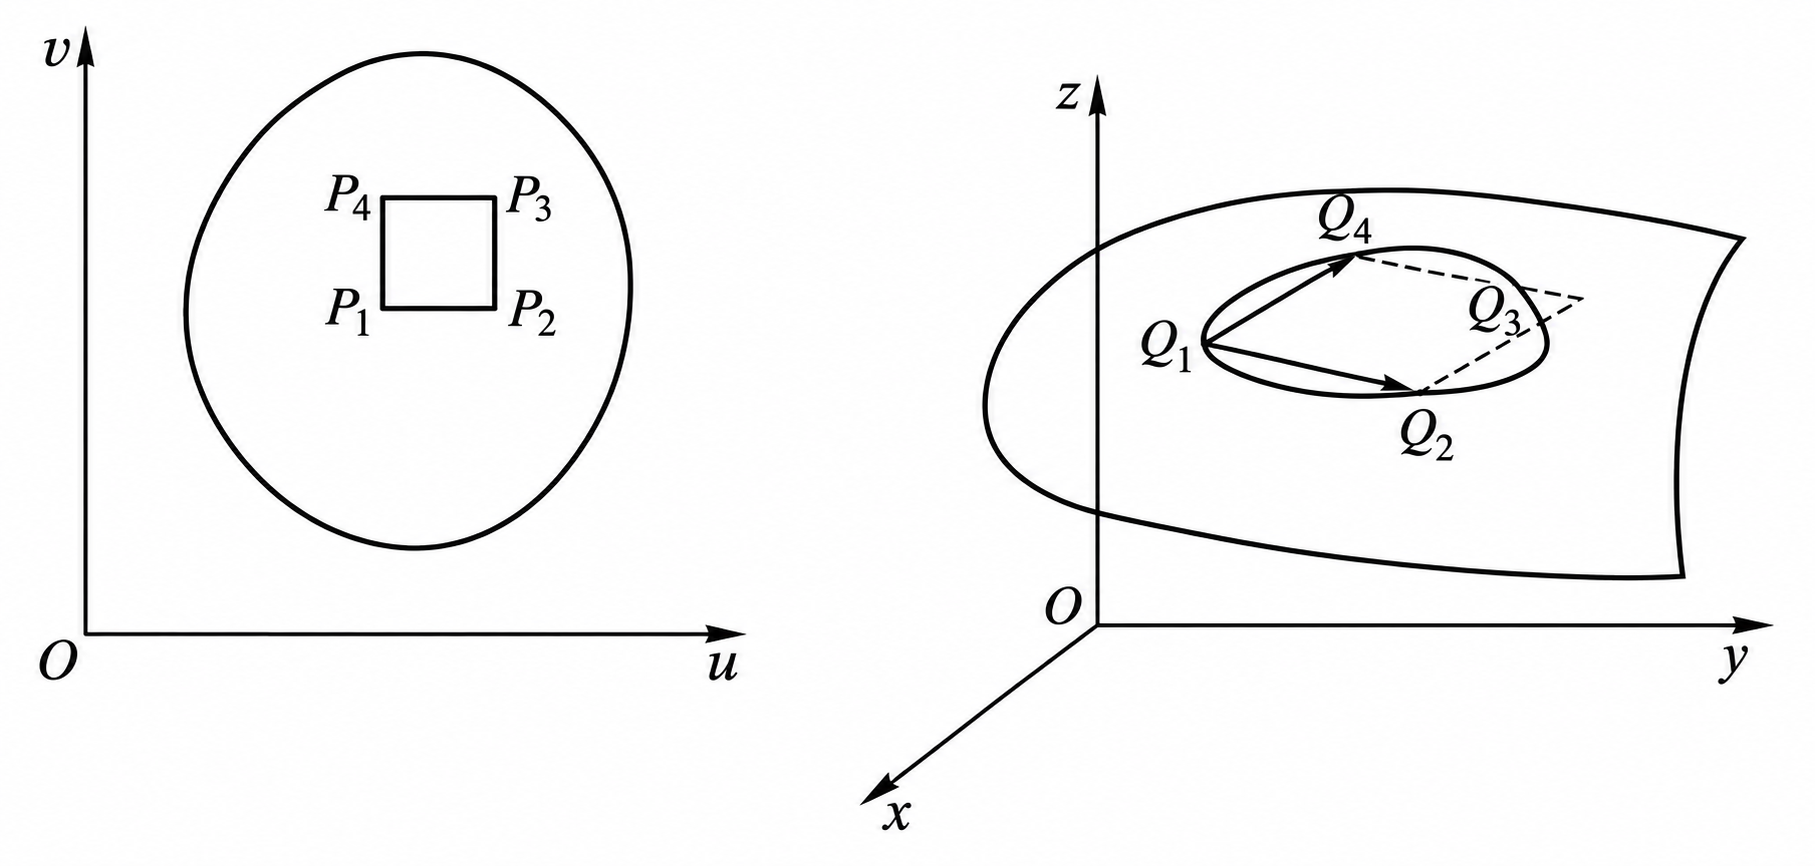
\includegraphics[width=0.78\linewidth]{figure/P2/fig14_1_3_redrawn_hd.png}
\end{center}
由中值定理，
\[
\begin{aligned}
\overrightarrow{Q_1Q_2}
&=\boldsymbol r(u_0+\Delta u,v_0)-\boldsymbol r(u_0,v_0)
=\boldsymbol r_u(u_0,v_0)\Delta u+o(\Delta u),\\
\overrightarrow{Q_1Q_4}
&=\boldsymbol r(u_0,v_0+\Delta v)-\boldsymbol r(u_0,v_0)
=\boldsymbol r_v(u_0,v_0)\Delta v+o(\Delta v).
\end{aligned}
\]
这里 $o(\Delta u),o(\Delta v)$ 表示模分别为 $\Delta u,\Delta v$ 的高阶无穷小的向量。小曲面片的面积可近似为切平面上以 $\boldsymbol r_u\Delta u$ 和 $\boldsymbol r_v\Delta v$ 为邻边的平行四边形的面积。因此曲面的面积微元和面积分别为
\[
\dd S=\lVert\boldsymbol r_u\times\boldsymbol r_v\rVert\,\dd u\dd v,\qquad
S=\displaystyle\iint_D\lVert\boldsymbol r_u\times\boldsymbol r_v\rVert\,\dd u\dd v.
\]
利用面积的可加性，这一方法可推广到由有限片这样的曲面拼成的分片光滑曲面。

\begin{theorem}
对上述曲面 $\Sigma$，记 Gauss 系数
\[
\begin{aligned}
E&=\boldsymbol r_u\cdot\boldsymbol r_u=x_u^2+y_u^2+z_u^2,\\
F&=\boldsymbol r_u\cdot\boldsymbol r_v=x_ux_v+y_uy_v+z_uz_v,\\
G&=\boldsymbol r_v\cdot\boldsymbol r_v=x_v^2+y_v^2+z_v^2.
\end{aligned}
\]
则曲面面积为
\[
S=\displaystyle\iint_D\sqrt{EG-F^2}\,\dd u\dd v.
\]
\end{theorem}
\begin{proof}
由外积的坐标表达式，
\[
\boldsymbol r_u\times\boldsymbol r_v
=\frac{\partial(y,z)}{\partial(u,v)}\boldsymbol i
+\frac{\partial(z,x)}{\partial(u,v)}\boldsymbol j
+\frac{\partial(x,y)}{\partial(u,v)}\boldsymbol k.
\]
因此
\[
\lVert\boldsymbol r_u\times\boldsymbol r_v\rVert^2
=\left(\frac{\partial(y,z)}{\partial(u,v)}\right)^2
+\left(\frac{\partial(z,x)}{\partial(u,v)}\right)^2
+\left(\frac{\partial(x,y)}{\partial(u,v)}\right)^2.
\]
将 $E,G,F$ 的表达式展开并合并同类项，得到同样的平方和，即
\[
EG-F^2=\lVert\boldsymbol r_u\times\boldsymbol r_v\rVert^2.
\]
代入曲面面积公式，即得结论。
\end{proof}

\begin{enumerate}
\item 若曲面方程为 $z=f(x,y)$，$(x,y)\in D$，其中 $f$ 具有连续偏导数，$D$ 是具有分段光滑边界的有界区域，则
\[
\boldsymbol r=x\boldsymbol i+y\boldsymbol j+f(x,y)\boldsymbol k,
\quad \boldsymbol r_x=\boldsymbol i+f_x\boldsymbol k,
\quad \boldsymbol r_y=\boldsymbol j+f_y\boldsymbol k.
\]
由 $EG-F^2=(1+f_x^2)(1+f_y^2)-f_x^2f_y^2=1+f_x^2+f_y^2$，得
\[
S=\displaystyle\iint_D\sqrt{1+f_x^2+f_y^2}\,\dd x\dd y.
\]
\item 若曲面方程为 $H(x,y,z)=0$，其中 $H$ 具有连续偏导数，且在曲面上 $H_z\ne0$；又设曲面在 $xy$ 平面上的投影将曲面一一对应地映为具有分段光滑边界的有界区域 $D$。由隐函数定理，曲面可表示为 $z=f(x,y)$，且
\[
f_x=-\frac{H_x}{H_z},\qquad f_y=-\frac{H_y}{H_z}.
\]
因此
\[
\begin{aligned}
S&=\displaystyle\iint_D\sqrt{1+\left(\frac{H_x}{H_z}\right)^2+\left(\frac{H_y}{H_z}\right)^2}\,\dd x\dd y\\
&=\displaystyle\iint_D\frac{\lVert\operatorname{grad}H\rVert}{|H_z|}\,\dd x\dd y.
\end{aligned}
\]
\end{enumerate}



\subsection*{Schwarz 的例子}
光滑曲线的弧长可以用内接折线长度的极限定义，但这一方法不能直接推广到曲面的面积：即使内接多面体各个三角形的直径都趋于零，其面积和也未必趋于曲面的面积。

设圆柱面的高为 $h>0$，半径为 $r>0$，其侧面积为 $2\pi rh$。在圆柱面上取三点 $A,B,C$，使 $A,B$ 在同一高度，$C$ 在另一高度，且 $C$ 在 $A,B$ 所在水平面上的投影 $C'$ 是短圆弧 $AB$ 的中点。连接 $A,B,C$，得到一个内接三角形。

将底圆 $m$ 等分，高 $n$ 等分；在各个水平截圆上取 $m$ 个等分点，相邻两层的等分点沿圆周错开半个分度，再连接相邻层的点，组成内接多面体的侧面。这样共有 $2mn$ 个全等三角形。
\begin{center}
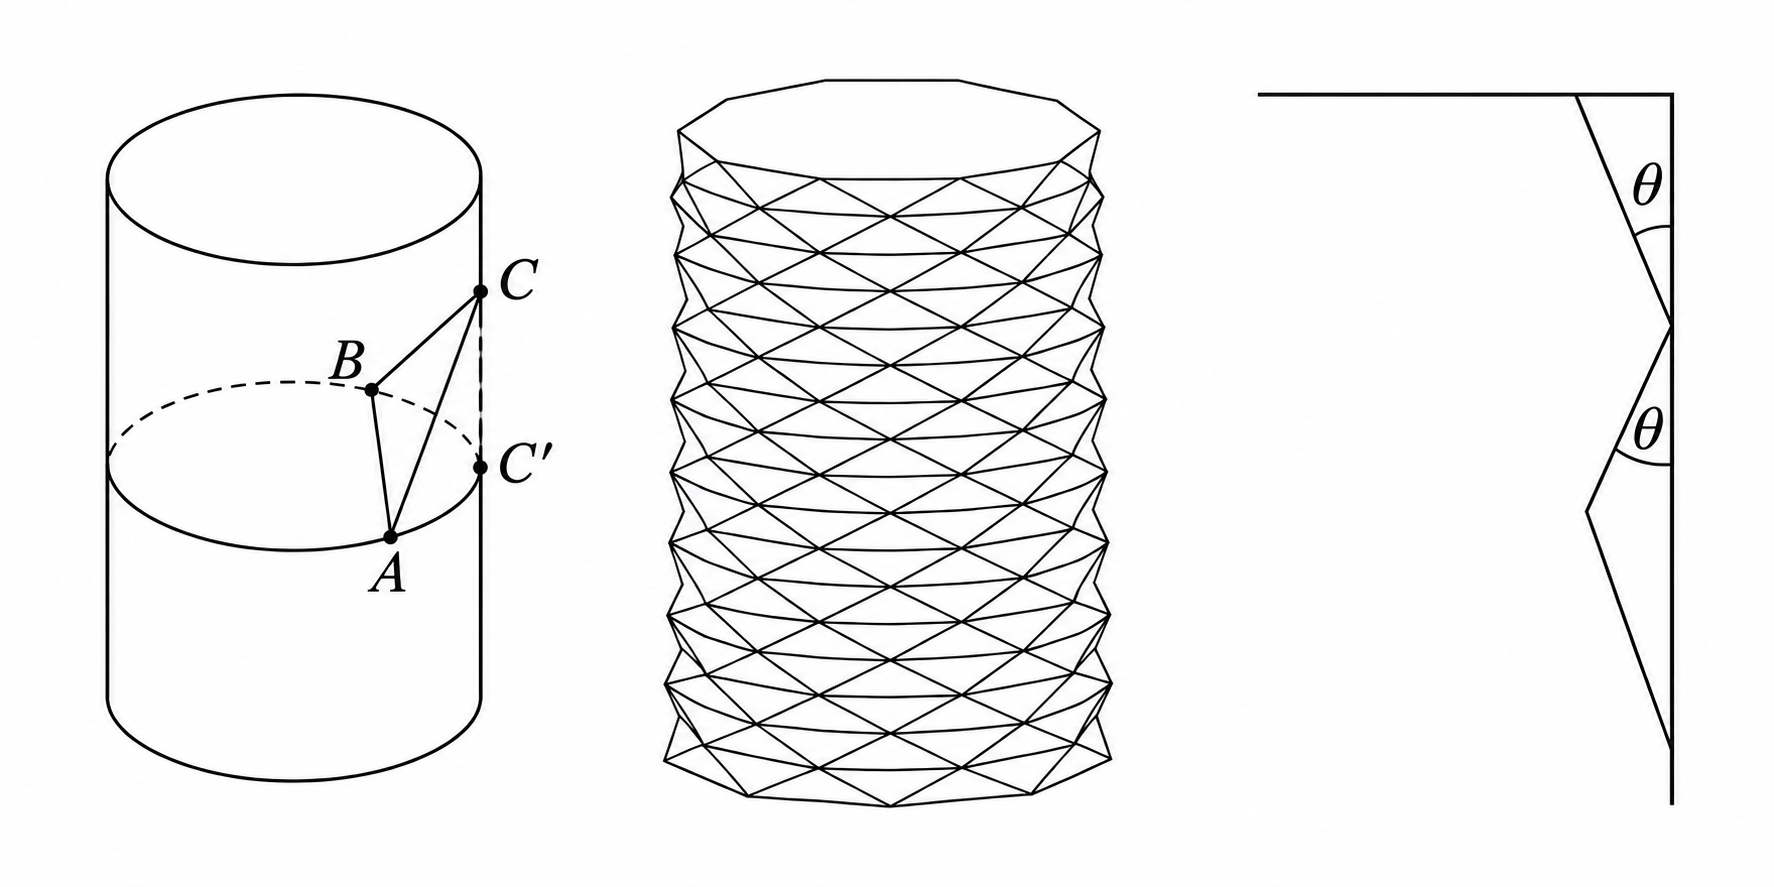
\includegraphics[width=0.95\linewidth]{figure/P2/schwarz_lantern_redrawn_hd.png}
\end{center}
每个三角形中，平行于底圆平面的底边长为
\[
b_m=2r\sin\frac{\pi}{m}.
\]
记底边中点为 $M$。由 $C'$ 是短圆弧 $AB$ 的中点，$C'M$ 垂直于弦 $AB$，且
\[
C'M=r\left(1-\cos\frac{\pi}{m}\right),\qquad CC'=\frac hn.
\]
又 $CC'$ 垂直于底圆平面，所以 $CM$ 是三角形 $ABC$ 的高，其长度为
\[
a_{m,n}=\sqrt{r^2\left(1-\cos\frac{\pi}{m}\right)^2+\frac{h^2}{n^2}}.
\]
由 $1-\cos t=2\sin^2(t/2)$，每个三角形的面积为
\[
\frac12 b_ma_{m,n}
=r\sin\frac{\pi}{m}\sqrt{4r^2\sin^4\frac{\pi}{2m}+\frac{h^2}{n^2}}.
\]
于是所有小三角形的面积之和为
\begin{align*}
S_{m,n}
&=2mnr\sin\frac{\pi}{m}\sqrt{4r^2\sin^4\frac{\pi}{2m}+\frac{h^2}{n^2}}\\
&=2\pi rh\frac{\sin(\pi/m)}{\pi/m}
\sqrt{1+\frac{\pi^4r^2}{4h^2}
\left(\frac{\sin(\pi/(2m))}{\pi/(2m)}\right)^4\frac{n^2}{m^4}}.
\end{align*}
当 $m,n\to\infty$ 时，各个三角形的直径确实趋于零：其底边长趋于零，另外两条边的长度均为
\[
\sqrt{4r^2\sin^2\frac{\pi}{2m}+\frac{h^2}{n^2}}\longrightarrow0.
\]
但面积和的极限取决于 $n/m^2$。若
\[
\frac{n}{m^2}\longrightarrow l\in[0,+\infty),
\]
则由 $\sin t/t\to1$，得到
\[
S_{m,n}\longrightarrow S(l)
=2\pi r\sqrt{h^2+\frac{\pi^4r^2l^2}{4}}.
\]
只有当 $l=0$ 时，这个极限才是圆柱面的侧面积 $2\pi rh$。例如，取 $n=m$ 时极限为 $2\pi rh$；取 $n=m^2$ 时极限严格大于 $2\pi rh$。若 $n/m^2\to+\infty$，则面积和趋于 $+\infty$。

因此，$m,n$ 同时趋于无穷的方式不同，面积和可以有不同的极限；仅要求小三角形的最大直径趋于零，不能用内接多面体面积的极限定义曲面面积。

再考察 $l=0$ 的几何意义。设 $\theta$ 为三角形所在平面与圆柱面在 $C'$ 处的母线的夹角。由于 $AB$ 垂直于由 $CC'$ 和 $C'M$ 张成的平面，在该截面内计算可得
\begin{align*}
\tan\theta
&=\frac{r-r\cos(\pi/m)}{h/n}
=\frac{2r\sin^2(\pi/(2m))}{h/n}\\
&=\frac{\pi^2r}{2h}
\left(\frac{\sin(\pi/(2m))}{\pi/(2m)}\right)^2\frac{n}{m^2}.
\end{align*}
所以，当 $n/m^2\to0$ 时，$\theta\to0$。在这一构造中，三角形平面含有与该处圆周切线平行的方向；因此 $\theta\to0$ 也表示三角形所在平面趋于相应的切平面。这与前面用切平面上的平行四边形计算面积微元的讨论相吻合。


\subsection*{第一类曲面积分}
\begin{definition}
设 $\Sigma$ 为有界光滑或分片光滑曲面，$f(x,y,z)$ 在 $\Sigma$ 上有界。用光滑曲线网将 $\Sigma$ 分成 $n$ 片小曲面 $\Delta\Sigma_1,\ldots,\Delta\Sigma_n$，记第 $i$ 片的面积为 $\Delta S_i$，并在其上任取一点 $(\xi_i,\eta_i,\zeta_i)$，作和式
\[
\sum_{i=1}^n f(\xi_i,\eta_i,\zeta_i)\Delta S_i.
\]
如果当所有小曲面直径的最大值 $\lambda\to0$ 时，这个和式的极限存在，且与划分及取点无关，就称该极限为 $f$ 在 $\Sigma$ 上的第一类曲面积分，记为
\[
\displaystyle\iint_\Sigma f(x,y,z)\,\dd S
=\lim_{\lambda\to0}\sum_{i=1}^n f(\xi_i,\eta_i,\zeta_i)\Delta S_i.
\]
其中 $f$ 称为被积函数，$\Sigma$ 称为积分曲面。
\end{definition}

设 $\Sigma$ 具有上面的参数表示，参数映射一一对应且满足前述光滑条件。如果 $f$ 在 $\Sigma$ 上连续，则第一类曲面积分存在，且
\[
\displaystyle\iint_\Sigma f(x,y,z)\,\dd S
=\displaystyle\iint_D f(x(u,v),y(u,v),z(u,v))\sqrt{EG-F^2}\,\dd u\dd v.
\]
特别地，若 $\Sigma$ 的方程为 $z=z(x,y)$，$(x,y)\in D$，则
\[
\displaystyle\iint_\Sigma f(x,y,z)\,\dd S
=\displaystyle\iint_D f(x,y,z(x,y))\sqrt{1+z_x^2+z_y^2}\,\dd x\dd y.
\]

% 原图未给出曲面积分计算公式的证明。
\begin{proof}
记 $g(u,v)=f(\boldsymbol r(u,v))$，$w(u,v)=\lVert\boldsymbol r_u\times\boldsymbol r_v\rVert$。对曲面的小片划分，记 $D_i$ 为 $\Delta\Sigma_i$ 在参数区域中的原像，并取 $p_i\in D_i$ 对应所选的曲面上的点。由曲面面积公式，
\[
\Delta S_i=\displaystyle\iint_{D_i}w(u,v)\,\dd u\dd v.
\]
于是相应的曲面积分和与右端积分之差为
\[
\sum_i f(\boldsymbol r(p_i))\Delta S_i
-\displaystyle\iint_D gw\,\dd u\dd v
=\sum_i\displaystyle\iint_{D_i}[g(p_i)-g(u,v)]w(u,v)\,\dd u\dd v.
\]
由于 $D$ 是紧集，连续单射 $\boldsymbol r:D\to\Sigma$ 的逆映射连续且一致连续。当曲面小片的最大直径趋于零时，各 $D_i$ 的直径也一致趋于零。又 $g$ 在 $D$ 上一致连续，所以
\[
\max_i\sup_{(u,v)\in D_i}|g(p_i)-g(u,v)|\longrightarrow0.
\]
上面差式的绝对值因此不超过这个最大值与曲面面积
$\displaystyle\iint_Dw\,\dd u\dd v$ 的乘积，故趋于零。这就证明了积分的存在性及计算公式。将 $\boldsymbol r(x,y)=(x,y,z(x,y))$ 代入即可得到特殊情形。
\end{proof}
